\vspace{10pt}

{\centering\subsection*{梁好:我最敬佩的人}}

\addcontentsline{toc}{subsection}{梁好:我最敬佩的人}

\renewcommand{\leftmark}{梁好:我最敬佩的人}

\begin{figure}[htbp]

\centering

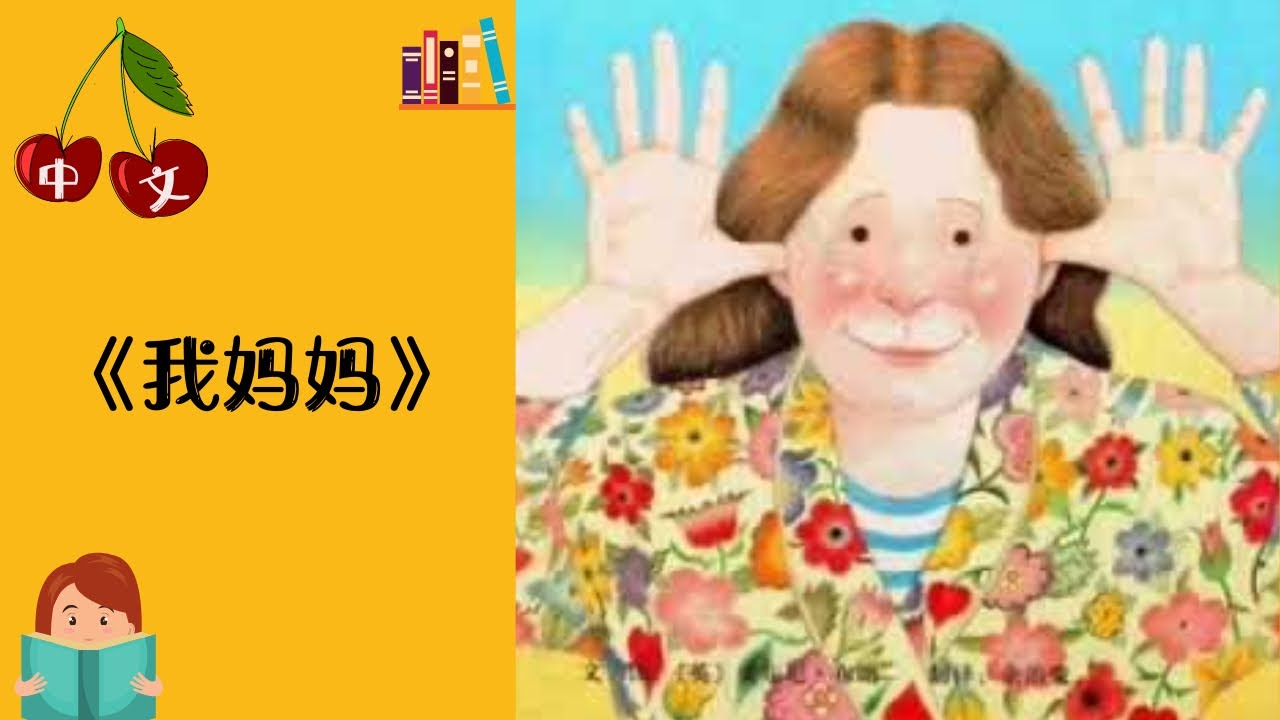
\includegraphics[width = .5\textwidth]{./ch/2.jpg}

\end{figure}





我最敬佩的人是我的妈妈,她有很多让我敬佩的事,今天我们就一起来看看吧!

他乐于助人的品质让我敬佩。比如每次看到大街上那些残疾人,睡大街的人,她总是会递上一个十几20块钱。我问妈妈为什么要给他们钱?妈妈便会对我说:“那些人生活不容易,也没收入,这几十元钱对我们家不是特别重要,但对别人来说就是救命的钱。”那时的我对妈妈无比的敬佩。

他面对困难时的办法也让我敬佩。有一个月家里比较困难。我妈妈没有选择逃避问题,而是勇敢的面对它,因为我妈妈知道逃避问题,只会让问题越来越大。她这种品质也让我们家从困难中走了出来。

她勇敢的品质也不得不让我敬佩。有一次我在姥姥家的菜地里玩,突然一条有着黑白色条纹的毒蛇,从草丛中爬了出来,我当时被吓的腿发软,根本走不动。我妈一下子冲过来抱起我赶紧跑开了。妈妈还差点被蛇咬到了,那时我对妈妈是无比的敬佩。

她热爱劳动的品质也让我钦佩。每天上班回到家,早就已经精疲力尽。妈妈回来却还要洗衣服,做饭,打扫卫生……可以说是干的没完没了,仿佛每天都有干不完的活和用不完的精力,她是那么用心,那时的她让我敬佩不已。

这就是我最敬佩的人——我的妈妈。她乐于助人,面对困难时的做法,勇敢、热爱劳动的品质,深深地影响了我。也照亮了我前行的路!





\vspace{10pt}



作者:四(1)班 梁好



指导老师:周瑞



投稿:2021年6月16日



发表:2021年6月17日






                



\vspace{10pt}

\hline



